\documentclass[handout]{beamer}
% L'option handout permet de supprimer la barre de navigation

\usepackage[T1]{fontenc}
\usepackage[utf8]{inputenc}
\usepackage[french]{babel}
% Pour utiliser le signe €
\usepackage{eurosym}
% Pour pouvoir insérer des images
\usepackage{graphicx}
\usepackage{wrapfig}
% Gestion des couleurs
\usepackage{color}
\definecolor{QTPurple}{RGB}{61, 68, 160} %3D44A0
% Coloration syntaxique
\usepackage{listings}

% Un joli thème flat
\usetheme{Rochester}

% Personnalisation du thème
\usecolortheme[named=QTPurple]{structure}
\setbeamertemplate{blocks}[shadow=false]

% ------------------------------------ %
% -- METADONNÉES DU DOCUMENT --------- %
\title[Stats]{
	Statistiques pour l'ingénieur\\
	Validation croisée
}
\author{
	Étienne Batise - Thibaud Dauce
}
\date{\today}

% \titlegraphic{\includegraphics[height=.3\textheight]{images/logo.png}}

% Début du document
\begin{document}
	
	% Génération de la page de titre
	\begin{frame}[plain]
		\titlepage
	\end{frame}

	% Génération du sommaire
	\begin{frame}[plain]
		\frametitle{Sommaire}
		\tableofcontents
	\end{frame}


	% ///////////////////////////////////////////////////////// %
	% /// Qu'est-ce que la validation croisée ? /////////////// %
	\section{Qu'est-ce que la validation croisée ?}

	\subsection{L'utilité}
		\begin{frame}
		\frametitle{L'utilité}
		\begin{tabular}{l l}
			\begin{minipage}{0.2\textwidth}
				\begin{center}
					
\includegraphics[width=0.9\textwidth]{images/cross.png}
				\end{center}
			\end{minipage}

			\begin{minipage}{0.8\textwidth}
				\begin{itemize}
					\item tester les données...
					\item ...avec peu de points
					\item ...sans faire trop de calculs
				\end{itemize}
			\end{minipage}

		\end{tabular}
		\end{frame}

	\subsection{Le principe}
		\begin{frame}
		\frametitle{Le principe}
		\begin{tabular}{l l}
			\begin{minipage}{0.5\textwidth}
				\begin{center}
					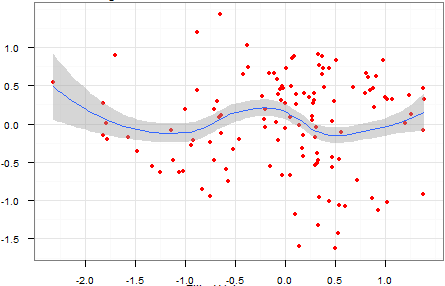
\includegraphics[width=0.8\textwidth]{images/function.png}
				\end{center}
			\end{minipage}

			\begin{minipage}{0.5\textwidth}
				\begin{itemize}
					\item après avoir trouvé la fonction
					\item tester sa validité
					\item deux groupes :
						\begin{itemize}
							\item groupe de données
							\item groupe de test
						\end{itemize}
				\end{itemize}
			\end{minipage}
			
		\end{tabular}
		\end{frame}

	\subsection{3 types de validation croisée}
		\begin{frame}
		\frametitle{3 types de validation croisée}
		\begin{tabular}{l l}
			\begin{minipage}{0.2\textwidth}
				\begin{center}
					
\includegraphics[width=0.9\textwidth]{images/clock.png}
				\end{center}
			\end{minipage}

			\begin{minipage}{0.8\textwidth}
				\begin{itemize}
					\item Rapport données / temps de calcul 
					\begin{itemize}
						\item testset validation
						\item k-fold cross-validation
						\item leave-one-out cross-validation
					\end{itemize}
				\end{itemize}
			\end{minipage}

		\end{tabular}
		\end{frame}

	% //////////////////////////////////////////// %
	% /// Démonstration ////////////////////////// %
	\section{Démonstration}

	\subsection{Présentation du code Octave}
		\begin{frame}
		\frametitle{Présentation}
		\begin{tabular}{l l}
			\begin{minipage}{0.4\textwidth}
				\begin{center}
					
\includegraphics[width=0.9\textwidth]{images/octave.png}
				\end{center}
			\end{minipage}

			\begin{minipage}{0.6\textwidth}
				\begin{itemize}
					\item génération de points aléatoires 
					\item calcul de la fonction par 3 méthodes 
					\item calcul de la validation croisée
				\end{itemize}
			\end{minipage}

		\end{tabular}
		\end{frame}

	% //////////////////////////////////////////// %
	% /// Le sytème d'information /////////////// %
	\section{Le sytème d'information}

	\subsection{Automatiser à l'extrême}
		\begin{frame}
		\frametitle{Automatiser à l'extrême}
		\begin{tabular}{l l}
			\begin{minipage}{0.2\textwidth}
				\begin{center}
					% \includegraphics[width=0.9\textwidth]{images/serveur.png}
				\end{center}
			\end{minipage}

			\begin{minipage}{0.8\textwidth}
				\begin{itemize}
					\item automatiser les adhésions
					\item automatiser l'assistance (hotline, tickets, incidents, brèves)
					\item outils de suivi : assistance et paiements
					\item de l'adhésion à la connexion fonctionnelle dans l'appartement : \mbox{\textbf{2 minutes}}
				\end{itemize}
			\end{minipage}
			
		\end{tabular}
		\end{frame}

	\subsection{L'assistance}
		\begin{frame}
		\frametitle{L'assistance}
		\begin{tabular}{l l}
			\begin{minipage}{0.2\textwidth}
				\begin{center}
					% \includegraphics[width=0.9\textwidth]{images/support.png}
				\end{center}
			\end{minipage}

			\begin{minipage}{0.8\textwidth}
				\begin{itemize}
					\item le plus coûteux en temps et en humain
					\item 90 \% des problèmes ne viennent pas de nous
					\item depuis septembre : 500 tickets / 300 appels
					\begin{itemize}
						\item problèmes d'infrastructure
						\item coupures de courant
						\item pertubations des ondes (Wi-Fi ou AirMax)
						\item prises RJ-45 mal câblées
					\end{itemize}
				\end{itemize}
			\end{minipage}
			
		\end{tabular}
		\end{frame}

	\subsection{Questions}
		\begin{frame}
		\frametitle{Questions}
		\huge{On vous écoute :)}
		\vspace{40px}
		\begin{center}
			% \includegraphics[height=.3\textheight]{images/logo.png}
		\end{center}
		\begin{center}
			\small{\underline{www.quantic-telecom.net}}
		\end{center}
		\end{frame}

	% ///////////////////////////////////////////////////////// %

% Fin du document
\end{document}
